\subsubsection{Pilot Interface and Control Systems}

The First-Person View (FPV) experience is defined by the synchronization between the pilot's inputs and the drone's visual feedback. An FPV drone can be controlled with a traditional remote controller or with a Motion Controller shown in \cref{fig:control}. A Motion Controller allows they user to maneuver the drone using hand gestures which is easy and convenient. The FPV Goggles is a also used for the FPV Drone. It's the defining factor for the FPV Drone. It connects to the drone's camera so that the camera user can have full vision of the quadcopter's camera \parencite{usama2021fpv}.


\begin{figure}[htbp]
    \centering
    \caption{Transmitter (Left) and Gamepad (Right)}\label{fig:control}
    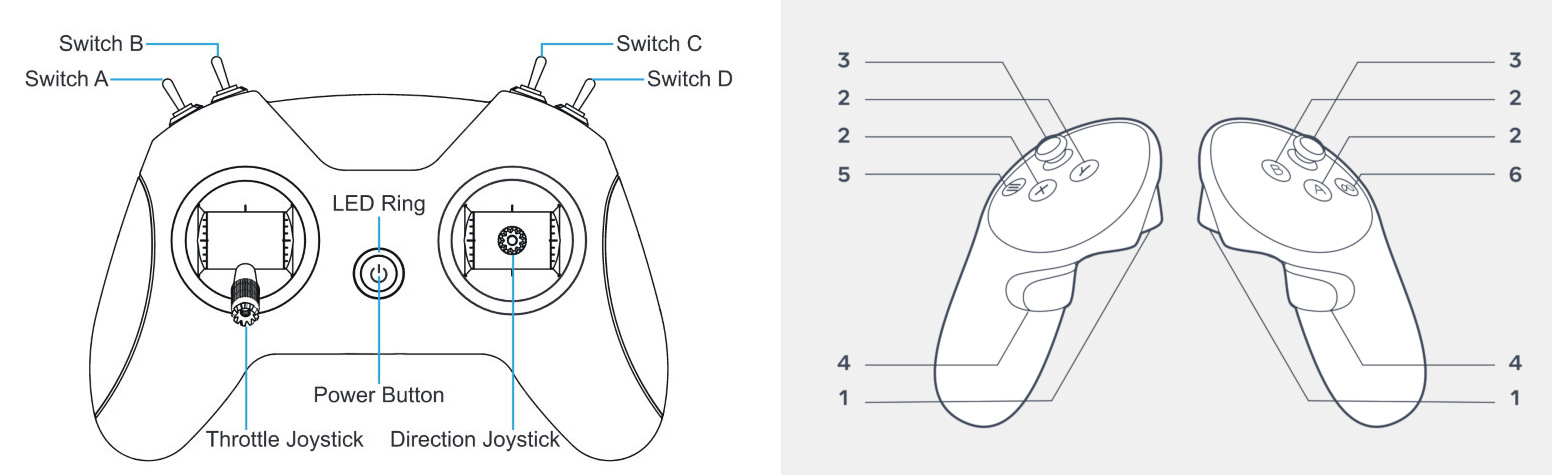
\includegraphics[width=0.8\linewidth]{img/control.jpg}
    \begin{flushleft}
    \small Adapted from \parencite{betafpv2022manual}
    \end{flushleft}
\end{figure}

The industry standardizes these controls into two primary layouts: Mode 1 (Japanese Hand): Predominantly used in Japan and parts of Europe. The throttle is located on the right gimbal; Mode 2 (American Hand): The global standard for FPV. The throttle is located on the left gimbal, which most pilots find more intuitive for separating altitude from directional pitch. Difference between Mode 1 and Mode 2 is shown in \cref{table:modes}

\begin{table}[h]
\caption{Comparison of Transmitter Control Modes}\label{table:modes}
\centering
\begin{tabular}{lllll}
\toprule
Mode & Left Stick (V) & Left Stick (H) & Right Stick (V) & Right Stick (H) \\
\midrule
Mode 1 & Pitch          & Yaw            & Throttle         & Roll            \\
Mode 2 & Throttle       & Yaw            & Pitch            & Roll            \\
\bottomrule
\end{tabular}
\end{table}

From a signal processing perspective, the flight controller differentiates between the unipolar throttle and the bipolar command sticks: Throttle ($T$): Mapped to a range of $[0, 1]$. Roll, Pitch, and Yaw ($\phi, \theta, \psi$): Mapped to a range of $[-1, 1]$. In \cref{fig:mode2} shows the interaction of the transmitter in Mode 2 and how the quadcopter move.

\begin{figure}
    \caption{Mode 2 control system}\label{fig:mode2}
    \centering
    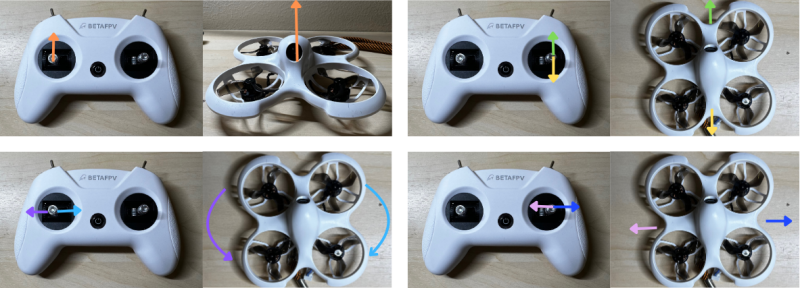
\includegraphics[width=0.8\linewidth]{img/drone.png}
    \begin{flushleft}
        \small Adapted from \parencite{betafpv2022manual}
    \end{flushleft}
\end{figure}


FPV drones generally operate across two flight logic modes. Self-Leveling (Angle/Normal Mode): The onboard flight controller uses accelerometers to automatically return the drone to a level horizon when the sticks are centered. This is ideal for beginners but limits maneuverability; Acrobat (Manual Mode): The controller only uses gyroscopes to maintain the current angular rate. If the pilot moves the stick and returns it to center, the drone maintains its current tilted orientation. This allows for flips and rolls but requires constant manual correction.

The FPV goggles provide the pilot with a low-latency first person view video feed pass from the camera set on the quadcopter's front. Beyond the video feed, an On-Screen Display (OSD) provides critical telemetry data, including battery voltage, signal strength, and flight time, as shown in \cref{fig:goggles}.

\begin{figure}
    \caption{The FPV goggles interface}\label{fig:goggles}
    \centering
    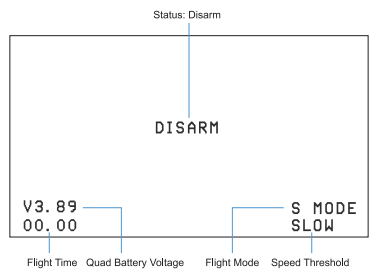
\includegraphics[width=0.8\linewidth]{img/goggles.png}
    \begin{flushleft}
        \small Adapted from \parencite{betafpv2022manual}
    \end{flushleft}
\end{figure}
